\documentclass[12pt]{article}

\usepackage{sbc-template}

\usepackage{graphicx,url}

%\usepackage[brazil]{babel}   
\usepackage[latin1]{inputenc}  


\sloppy

\title{Bat Algorithm on GPU}

\author{Jean Carlo Machado\inst{1}}

\address{ Universidade Estadual de Santa Catarina
  (UDESC) Joinville, SC.
}

\begin{document}

\maketitle

\begin{abstract}
\end{abstract}

\begin{resumo} 
\end{resumo}


\section{General Information}

The bat algorithm was introduced...

In this work the bath algorithm used was the one proposed by (parpinelli reference).

It was developed two versions of the algorithm. One that runs on CPU and the other which uses CPU.



The benchmark functions used were the following:

ROSENBROOK, SPHERE, SCHWEFEL, ACKLEY, RASTRINGIN, GRIEWANK, SHUBER

For the GPU version the approach used was the split of each individual in one thread.
It was observed speedups with big populations.


The tests were executed on an I5 with...



% Figure and table captions should be centered if less than one line
% (Figure~\ref{fig:exampleFig1}), otherwise justified and indented by 0.8cm on
% both margins, as shown in Figure~\ref{fig:exampleFig2}. The caption font must
% be Helvetica, 10 point, boldface, with 6 points of space before and after each
% caption.

% \begin{figure}[ht]
% \centering
% 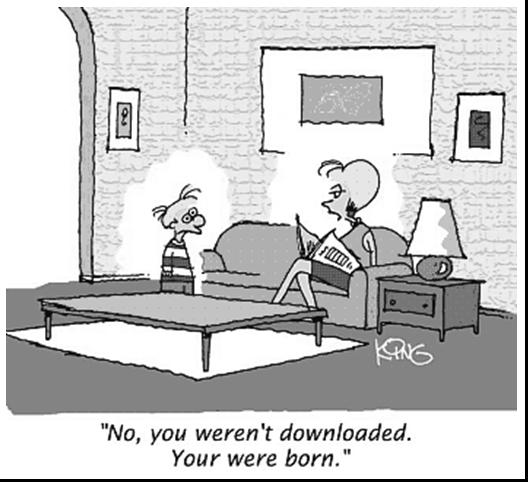
\includegraphics[width=.5\textwidth]{fig1.jpg}
% \caption{A typical figure}
% \label{fig:exampleFig1}
% \end{figure}

% \begin{figure}[ht]
% \centering
% 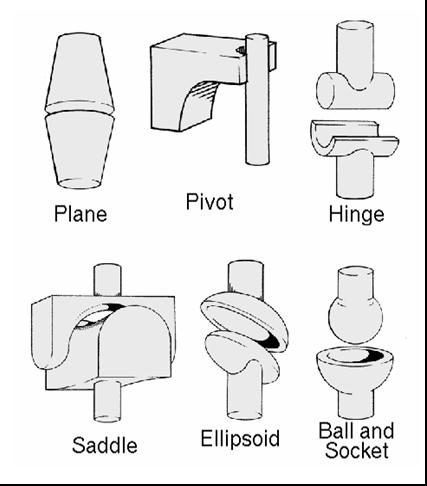
\includegraphics[width=.3\textwidth]{fig2.jpg}
% \caption{This figure is an example of a figure caption taking more than one
%   line and justified considering margins mentioned in Section~\ref{sec:figs}.}
% \label{fig:exampleFig2}
% \end{figure}

% In tables, try to avoid the use of colored or shaded backgrounds, and avoid
% thick, doubled, or unnecessary framing lines. When reporting empirical data,
% do not use more decimal digits than warranted by their precision and
% reproducibility. Table caption must be placed before the table (see Table 1)
% and the font used must also be Helvetica, 10 point, boldface, with 6 points of
% space before and after each caption.

% \begin{table}[ht]
% \centering
% \caption{Variables to be considered on the evaluation of interaction
%   techniques}
% \label{tab:exTable1}
% 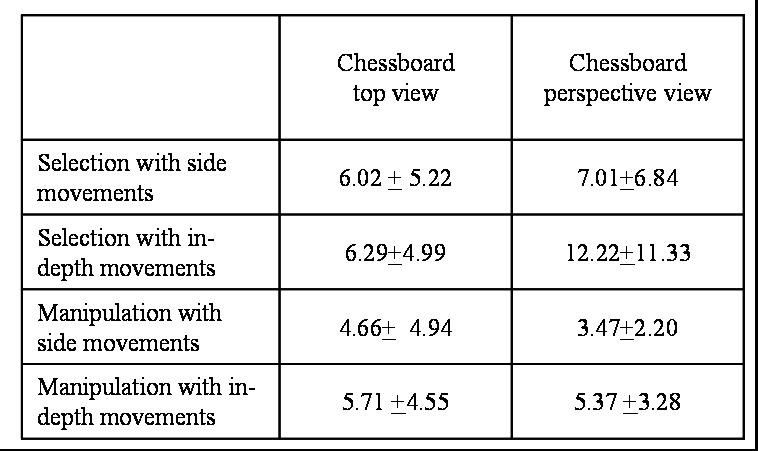
\includegraphics[width=.7\textwidth]{table.jpg}
% \end{table}

% \section{Images}

% All images and illustrations should be in black-and-white, or gray tones,
% excepting for the papers that will be electronically available (on CD-ROMs,
% internet, etc.). The image resolution on paper should be about 600 dpi for
% black-and-white images, and 150-300 dpi for grayscale images.  Do not include
% images with excessive resolution, as they may take hours to print, without any
% visible difference in the result. 

\section{References}

Bibliographic references must be unambiguous and uniform.  We recommend giving
the author names references in brackets, e.g. \cite{knuth:84},
\cite{boulic:91}, and \cite{smith:99}.

The references must be listed using 12 point font size, with 6 points of space
before each reference. The first line of each reference should not be
indented, while the subsequent should be indented by 0.5 cm.

\bibliographystyle{sbc}
\bibliography{sbc-template}

\end{document}
